\section{Summary Generation in the Mrs. Pacman Domain}
\label{sec:pacman}
We used HIGHLIGHTS to generate summaries for agents playing the Mrs. Pacman game~\cite{rohlfshagen2011ms}. Figure~\ref{fig:pacman} shows the game maze used in our experiments. This game configuration includes two types of food pellets: regular pellets (small dots) are worth 10 points each and power pellets (larger dots) are worth 50 points each. After eating a power pellet, ghosts become edible for a limited time period. Pac-Man receives 200 points for each ghost it eats. Ghosts chase Pac-Man with $80\%$ probability and otherwise move randomly. In each state, Pac-Man has at most four moves (right, left, up or down). 

\begin{figure}
	\centering
	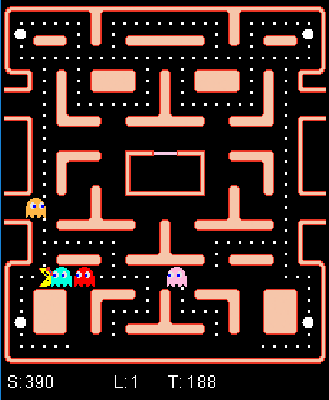
\includegraphics[width=0.4\columnwidth]{figs/pacman1.pdf}\\
	\caption{The Mrs. Pac-Man Game.}
	\label{fig:pacman}
	\vspace{-0.4cm}
\end{figure}

Due to the large size of the state space, we used a high-level feature representation for state-action pairs. Specifically, we use the 7-feature representation from Torrey \& Taylor's~\shortcite{torrey2013teaching} implementation. Q-values are defined as a weighted function of the feature values $ f_{i}(s,a)$:
\begin{equation}
Q(s,a)=\omega_{0}+\sum_{i}{\omega_{i} \cdot f_{i}(s,a)}
\label{e:q}
\vspace{-0.3cm}
\end{equation}

To generate Pacman agents of varying capabilities, we run the SARSA reinforcement learning algorithm with varying number of training episodes. We generated 3 different agents: (1) an agent trained for 200 episodes; (2) an agent trained for 400 episodes, and (3) an agent trained for 2000 episodes. We chose these thresholds as they empirically resulted in differing qualitative performance. For example, the agent trained for 2000 episodes learned that eating ghosts provides a large reward, while the other two did not. 